\section*{Exercise 5}
\subsection*{a)}
The Markov Chain for the sudents behaviour can be described by the following graph:
\begin{center}
  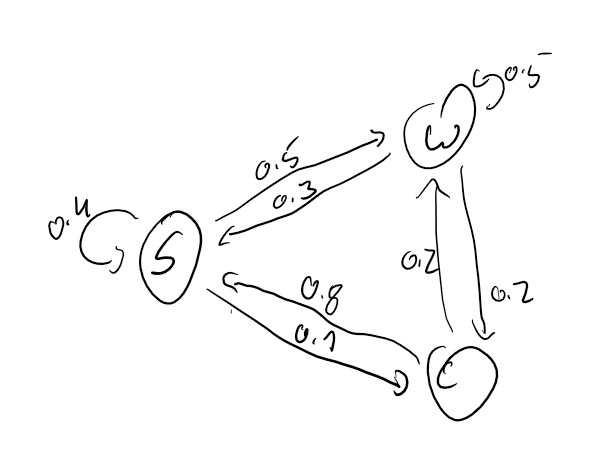
\includegraphics[scale = 0.75]{EX5Graph.png}
\end{center}
\subsection*{b)}
We can derive the transition matrix \[\mathcal{Q} = \left(\begin{matrix}
0.4&0.5&0.1\\0.3&0.5&0.2\\0.8&0.2&0
\end{matrix}\right)\]
The initial distribution is the distribution after leaving the state $c$. So $p_0 = \left(\begin{matrix}
0.8&0.2&0
\end{matrix}\right)$.
From this distribution the propability distribution after 2 hours can be dervied:
\[p_2 = p_0 * \mathcal{Q}^2 = \left(0.398\:0.464\:0.138\right)\]
Therefore the proibaility of the student starting to clean two hours later is $13.8\%$.

\subsection*{c)}
To find the long-term fraction of time the student is studying we need to find the stationary distribution of the Markov Chain.
The Martkov Chain obviously is ergodic.
Therefore we can find a stationary distribution $\pi$ by calculating $p_t = p_0 * \mathcal{Q}^t$ for any starting distribution until $p_t = p_{t+1}$.
\begin{center}
  \begin{tabular}{r|c}
    $t$&$p_t$\\\hline
    0&$(0.398\; 0.464\;0.138)$\\
    1&$(0.4088\; 0.4586\;0.1326)$\\
    2&$(0.40718\; 0.46022\;0.1326)$\\
    3&$(0.407018\; 0.46022\;0.1326762)$\\
    4&$(0.407083\; 0.460171\;0.1326746)$\\
    5&$(0.407081\; 0.460176\;0.1326743)$\\
    6&$(0.407079\; 0.460177\;0.1326743)$\\
    7&$(0.407078\; 0.460177\;0.1326743)$\\
    8&$(0.407078\; 0.460177\;0.1326743)$\\
  \end{tabular}
\end{center}
The fraction of time the student is studying in the long run is eqivalent to the stationary propability of the student choosing to study wich is $40.708\%$.